% ==============================================
% CFD Tutorial Template: OpenFOAM Terminal Basics
% Class: scrartcl (KOMA-Script) - optimized for tutorials
% Content: pitzDaily with FreeCAD
% ==============================================

\documentclass[
    parskip=half,      % Space between paragraphs (better for steps)
    DIV=12,            % Optimal margins for readability
    headings=normal,   % Professional heading sizes
    fontsize=11pt,     % Slightly larger for screen reading
    english            % Language setting
]{scrartcl}

% ========== ESSENTIAL PACKAGES ==========
\usepackage[utf8]{inputenc}
\usepackage[T1]{fontenc}
\usepackage{lmodern}
\usepackage{geometry}
\usepackage{tikz}
\usepackage{microtype}           % Superior typography
\usepackage{graphicx}            % For screenshots (optional)
\usepackage{xcolor}              % Color coding
\usepackage{listings}            % Code listings
\usepackage{siunitx}             % Proper units: \si{\meter\per\second}
\usepackage{amsmath}             % Math equations
\usepackage{hyperref}            % Clickable links
\usepackage{url}
\usepackage{booktabs}            % Professional tables
\usepackage{caption}             % Better figure captions
\usepackage[english]{babel}
\usepackage{float}

% ========== CUSTOM COLORS ==========
\definecolor{codebg}{RGB}{240, 245, 250}
\definecolor{cmdcolor}{RGB}{0, 100, 0}
\definecolor{outputcolor}{RGB}{100, 100, 150}
\definecolor{warningcolor}{RGB}{180, 0, 0}
\definecolor{tipcolor}{RGB}{0, 100, 50}

% ========== CODE LISTING SETUP ==========
\lstset{
	backgroundcolor=\color{codebg},
	basicstyle=\ttfamily\small,
	breaklines=true,
	frame=single,
	captionpos=b,
	rulecolor=\color{gray!30},
	tabsize=2,
	showstringspaces=false
}

% Custom style for terminal commands
\lstdefinestyle{terminal}{
	basicstyle=\ttfamily\small\color{cmdcolor},
	backgroundcolor=\color{black!5},
	frame=none,
	columns=fullflexible
}

% Custom style for OpenFOAM files
\lstdefinestyle{openfoam}{
	language=C++,
	morekeywords={dimensions, internalField, boundaryField, type, value},
	keywordstyle=\color{blue},
	commentstyle=\color{gray!50}\itshape
}

\lstdefinestyle{output}{
	backgroundcolor=\color{black!5},
	basicstyle=\ttfamily\small\color{outputcolor},
	frame=none,
	breaklines=true
}
% ========== HYPERREF SETUP ==========
\hypersetup{
	colorlinks=true,
	linkcolor=blue,
	citecolor=green,
	filecolor=magenta,
	urlcolor=cyan,
	pdftitle={OpenFOAM Tutorial: pitzDaily with simpleFoam},
	pdfauthor={Your Name},
	pdfsubject={CFD with OpenFOAM},
	pdfkeywords={OpenFOAM, CFD, simpleFoam, pitzDaily, terminal}
}


\newcommand{\warning}[1]{\par\vspace{5pt}\noindent\textcolor{red}{\textbf{WARNING:}} #1\par\vspace{3pt}}
\newcommand{\tip}[1]{\par\vspace{5pt}\noindent\textcolor{green!50!black}{\textbf{TIP:}} #1\par\vspace{3pt}}
\newcommand{\important}[1]{\par\vspace{5pt}\noindent\textcolor{blue}{\textbf{IMPORTANT:}} #1\par\vspace{3pt}}                    

% ========== CUSTOM COMMANDS ==========
\newcommand{\terminalcmd}[1]{\textbf{\texttt{\textcolor{cmdcolor}{#1}}}}
\newcommand{\ofkeyword}[1]{\textbf{\textcolor{blue}{#1}}}
\newcommand{\filename}[1]{\texttt{\textcolor{purple}{#1}}}
\newcommand{\commandexample}[1]{\vspace{5pt}\hspace{10pt}\terminalicon\ \terminalcmd{#1}\vspace{5pt}}
\newcommand{\key}[1]{\texttt{\textbf{#1}}}


% ========== DOCUMENT START ==========
\begin{document}

% ========== TITLE PAGE ==========
\title{Tutorial \#2: OpenFOAM with FreeCAD}
\subtitle{Incompressible Steady Flow: pitzDaily with FreeCAD - CfdOf}
\subject{Open Source CFD }
\author{Robert Castilla \\ Department of Fluid Mechanics}
\date{2025-26 \\ Version 1.0}
\publishers{Learning Objectives:
\begin{itemize}
    \item Create 3D geometry with FreeCAD
    \item Setup CFD simulation in FreeCAD with CfdOf
    \item Generate volume mesh % with boundary layers
    \item Setup Boundary Conditions
    \item Run Solver ion FreeCAD
    \item PostProcessing with paraview
\end{itemize}}

\maketitle

% ========== ABSTRACT ==========
\begin{abstract}
This tutorial introduces the fundamental workflow of Computational Fluid Dynamics (CFD) using OpenFOAM in a FreeCAD with the CfdOf workbench. Through the classic \filename{pitzDaily} case, students will learn to set up, run, and analyze an incompressible steady-state flow simulation. The postprocessing, like in Tutorial 1, will
be done with paraview.
\end{abstract}

\tableofcontents
\newpage

% ========== SECTION 1: INTRODUCTION ==========
\section{Introduction and Theoretical Background}

\subsection{What is pitzDaily?}
The \filename{pitzDaily} case simulates 2D steady, turbulent flow in a backward-facing step configuration. It's included in the OpenFOAM tutorials and serves as an excellent starting point due to its:
\begin{itemize}
    \item Simple geometry but interesting physics (recirculation zone)
    \item Complete setup with all necessary files
    \item Quick runtime (minutes on most computers)
\end{itemize}

\begin{figure}[h]
	\begin{center}
		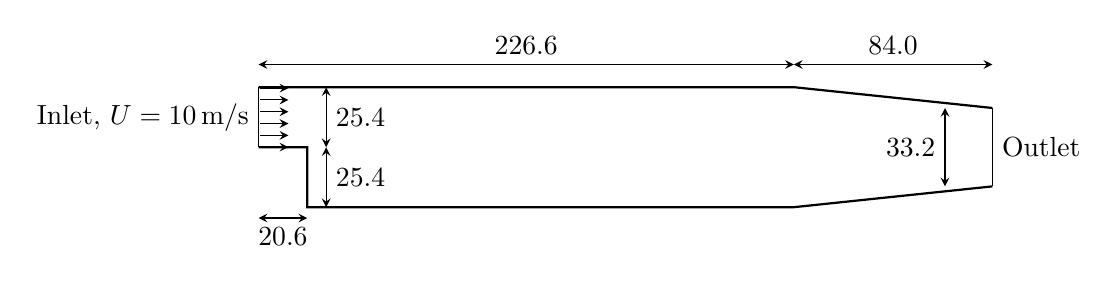
\begin{tikzpicture}[scale=0.03]
	% Draw the backward-facing step geometry
	\draw[thick] (-20.6,0) -- (0,0) -- (0,-25.4) -- (206,-25.4) -- (290,-16.6); % Lower
	\draw[thick] (-20.6,25.4) -- (0,25.4) -- (206,25.4) -- (290,16.6); % Upper
	\draw[thin] (-20.6,0) -- (-20.6,25.4) node[midway, left]{Inlet, $U = \qty{10}{m/s}$}; % Inlet
	\draw[thin] (290,-16.6) -- (290,16.6) node[midway, right]{Outlet}; % Outlet
	
	% Flow direction
	\foreach \y in {-0, 5, 10, 15, 20, 25} 
	\draw[-stealth] (-20,\y) -- ++(12,0);
	
	% Dimensions
	\draw[thin,stealth-stealth] (-20.6,35) -- (206,35) node[midway, above]{226.6}; 
	\draw[thin,stealth-stealth] (206,35) -- (290,35) node[midway, above]{84.0};
	\draw[thin,stealth-stealth] (270,-16.6) -- (270,16.6) node[midway, left]{33.2};
	\draw[thin,stealth-stealth] (8,0) -- (8,25.4) node[midway, right]{25.4};
	\draw[thin,stealth-stealth] (8,0) -- (8,-25.4) node[midway, right]{25.4};
	\draw[thin,stealth-stealth] (-20.6,-30) -- (0,-30) node[midway, below]{20.6};
\end{tikzpicture}
	\end{center}
	\caption{pitzDaily geometry. Lengths are in millimeter.}
	\label{fig:geometry}
\end{figure}

\subsection{Governing Equations}
The \terminalcmd{simpleFoam} solver implements the incompressible Reynolds-Averaged Navier-Stokes (RANS) equations:

\begin{equation}
\nabla \cdot \mathbf{U} = 0
\end{equation}

\begin{equation}
\nabla \cdot (\mathbf{U} \mathbf{U})  = -\nabla p + \nabla \cdot (\nu_{\text{eff}} \nabla \mathbf{U})
\end{equation}

where $\nu_{\text{eff}} = \nu + \nu_t$ is the effective viscosity (molecular + turbulence viscosity).

\newpage

\subsection{Case Overview}
\begin{table}[h]
\centering
\begin{tabular}{@{}ll@{}}
\toprule
\textbf{Parameter} & \textbf{Value} \\
\midrule
Solver & \terminalcmd{simpleFoam} (steady, incompressible) \\
Turbulence model & $k$-$\epsilon$ (standard) \\
Flow regime & Turbulent \\
Geometry & 2D backward-facing step \\
Reynolds number & $\sim 2 \times 10^4$ (based on step height) \\
Expected runtime & 5-10 seconds \\
\bottomrule
\end{tabular}
\caption{pitzDaily case specifications}
\label{tab:case_specs}
\end{table}

% ========== SECTION 2: FreeCAD Environment ==========
\section{FreeCAD Environment Setup}

\subsection{What is FreeCAD and CfdOf}

\href{https://www.freecad.org}{FreeCAD} is a free, open-source parametric 3D CAD modeler with a modular architecture. It is extensible through workbenches. 

\href{https://github.com/jaheyns/CfdOF}{CfdOf} is an workbench for FreeCAD 
which provides a basic CFD workflow.  

CfdOf is not installed in FreeCAD by default. Instructions for the installation can be 
found in its home page.

Figure \ref{fig:freecad001} show the startup window of FreeCAD. 

\begin{figure}[h]
	\centering
	\includegraphics[width=0.8\linewidth]{FreeCAD001}
	\caption{Startup screen of FreeCAD}
	\label{fig:freecad001}
\end{figure}

\subsection{Basic setup}

By default, FreeCAD is configured to work with millimeters. Since natural OpenFOAM
system of units is the International one, the first task is not change the default unit 
system. To do that, navigate to  
\ofkeyword{Edit $\rightarrow$ Preferences $\rightarrow$ General} and change the default 
unit system to meters.

% ========== SECTION 3: GEOMETRY ==========
\section{3D Geometry generation}

Clik on \ofkeyword{New} to create a new document. By default, the 
\ofkeyword{Part Design} workbench is activated.

Click on \ofkeyword{sketch} button (see Figure \ref{fig:freecad002}) to create a new sketch

\begin{figure}[H]
	\centering
	\includegraphics[width=0.8\linewidth]{FreeCAD002}
	\caption{To make the initial sketch}
	\label{fig:freecad002}
\end{figure}

Select plane XY and click \ofkeyword{OK}.

Loosely draw a polyline following the shape of the pitzDaily geometry 
(Figure \ref{fig:geometry}). Don't worry about 
constraints and dimension; it will be defined later (Figure \ref{fig:freecad003}).

\begin{figure}[H]
	\centering
	\includegraphics[width=0.8\linewidth]{FreeCAD003}
	\caption{The sketch, without correct dimensions}
	\label{fig:freecad003}
\end{figure}

Now the correct dimensions can be defined with the constraints tools. When the 
constraints are right, the sketch becomes \textcolor{green}{green} (Figure \ref{fig:freecad004}).

\begin{figure}[H]
	\centering
	\includegraphics[width=0.8\linewidth]{FreeCAD004}
	\caption{Sketch with dimensions and constraints.}
	\label{fig:freecad004}
\end{figure}

The sketch can be closed by clicking \ofkeyword{Close}. The last step is to
extrude this sketch with the \ofkeyword{Pad} tool. Choose a length of 4 mm (Figure \ref{fig:freecad005})

\begin{figure}[h]
	\centering
	\includegraphics[width=0.8\linewidth]{FreeCAD005}
	\caption{3D part for the pitzDaily geometry.}
	\label{fig:freecad005}
\end{figure}




% ========== SECTION 3: CFD ==========
\section{CFD simulation with CfdOF}


\subsection{First steps}

Select the \ofkeyword{CfdOF} workbench and, with the \ofkeyword{Pad} selected, click on 
the \ofkeyword{Analisys Container} icon. 

\begin{figure}[H]
	\centering
	\includegraphics[width=0.8\linewidth]{FreeCAD006}
	\caption{CfdOF workbench and analysis container}
	\label{fig:freecad006}
\end{figure}


\ofkeyword{CfdOF} will create the OpenFOAM case on disk in order to make the simulation. 
By default, the cases are stored in the \filename{/tmp} folder. Change this default folder 
to \filename{\textasciitilde/Tutorials/Tutorial\_2} in \ofkeyword{CfdOF $\rightarrow$ Open preferences 
$\rightarrow$ Default output directory}. Make the folder, if necessary. Click \ofkeyword{OK}
to save the options and close the preferences window.


Expand the \ofkeyword{CfdAnalysis}, and double-click on \ofkeyword{Physics model}. Select:
\begin{itemize}
	\item Steady
	\item Single phase
	\item Isothermal
	\item Viscous
	\item RANS $\rightarrow$ kOmegaSST
\end{itemize}

The window can be closed with \ofkeyword{OK}.

Double-click on \ofkeyword{Fluid Properties} and click on \ofkeyword{OK} to 
select \ofkeyword{Air}, the default option.


\subsection{Setup of boundary conditions and mesh}

Select the face for the inlet and click on the icon for \ofkeyword{Fluid boundary}.



\begin{figure}[H]
	\centering
	\includegraphics[width=0.8\linewidth]{FreeCAD007}
	\caption{Selection of the inlet boundary condition.}
	\label{fig:freecad007}
\end{figure}

Define the boundary with:

\begin{itemize}
	\item Boundary: \ofkeyword{Inlet}
	\item Sub-type: \ofkeyword{Uniform velocity}
	\item Velocity: 10 m/s in the X direction
	\item Pressure: 100 kPa
	\item Turbulence specifications:
	\begin{itemize}
		\item TKE (k) : 0.375 m\textasciicircum 2/s\textasciicircum 2
		\item SDR ($\omega$) : 440.15 Hz
	\end{itemize}
\end{itemize}

Click \ofkeyword{OK} to define the inlet boundary condition.

Repeat the process for

\begin{description}
	\item[outlet:] 1 face. Boundary \ofkeyword{Outlet}, Sub-type \ofkeyword{Static Pressure},
	with pressure \qty{0}{kPa} (relative pressure).
	\item[wall:] 6 faces. Several faces can be selected with the \terminalcmd{Ctrl} key. 
	Boundary \ofkeyword{Wall}, Sub-type \ofkeyword{No-slip}.
	\item[constraint:] 2 faces, normal to Z direction. Boundary \ofkeyword{Constraint}, Sub-type \ofkeyword{Symmetry}
\end{description}

Make the mesh by selecting the \ofkeyword{Pad} and clicking on the \ofkeyword{CFD mesh} 
icon

\begin{figure}[H]
	\centering
	\includegraphics[width=0.8\linewidth]{FreeCAD007b}
	\caption{Making the mesh}
	\label{fig:freecad007b}
\end{figure}

Keep \ofkeyword{cfMesh} as mesh utility, and write \terminalcmd{1 mm} as  
\ofkeyword{Base element size}. Write the mesh case on disk. If desired, the mesh case can 
be explored and edited. Generate the mesh with \ofkeyword{Run mesher}. It will take just 
some seconds. The mesh can be visualized directly in FreeCAD with \ofkeyword{Load surface
mesh} (Figure \ref{fig:freecad007c}) or with \ofkeyword{ParaView} 
(Figure \ref{fig:paraview001}).

\begin{figure}[H]
	\centering
	\includegraphics[width=0.8\linewidth]{FreeCAD007c}
	\caption{Mesh visualized in FreeCAD}
	\label{fig:freecad007c}
\end{figure}

\begin{figure}[H]
	\centering
	\includegraphics[width=0.8\linewidth]{ParaView001}
	\caption{Mesh visualized with ParaView.}
	\label{fig:paraview001}
\end{figure}

Finally, since the solver is an iterative process, an initial state of the problem has to 
be provided. It is done with the \ofkeyword{InitialiseFields} icon 
(Figure \ref{fig:freecad007d}).

\begin{figure}[H]
	\centering
	\includegraphics[width=0.8\linewidth]{FreeCAD007d}
	\caption{Icon to initialise the fields for the iterative computation.}
	\label{fig:freecad007d}
\end{figure}

For \textbf{velocity}, keep the potential flow. For \textbf{pressure} 
use the value from the \ofkeyword{outlet} boundary, and for \textbf{turbulence}, 
from the \ofkeyword{inlet} one. 
Click \ofkeyword{OK}.

\subsection{Running the Simulation}

Before running the solver, the program has to be setup to use only one processor. 

\begin{figure}[H]
	\centering
	\includegraphics[width=0.8\linewidth]{FreeCAD008}
	\caption{Selection of one core for serial simulation.}
	\label{fig:freecad008}
\end{figure}


To run the solver, double-click on the icon \ofkeyword{Cfdsolver}, and write the case 
to the disk.

Click on the \ofkeyword{Run} button and the \textbf{Residuals} of the equations 
will be visualised on the screen.

\begin{figure}[H]
	\centering
	\includegraphics[width=0.8\linewidth]{Residuals001}
	\caption{Residuals of the equations in the iterative process.}
	\label{fig:residuals001}
\end{figure}

The simulation will stop when all the residuals reach a value below \num{e-3}

\section{Post-processing}

The results of the simulation can be processed with \ofkeyword{ParaView}, 
in the some way as in Tutorial 1.

\begin{figure}[H]
	\centering
	\includegraphics[width=0.8\linewidth]{ParaView002}
	\caption{Simulation results in \ofkeyword{ParaView}.}
	\label{fig:paraview002}
\end{figure}

When \ofkeyword{CfdOf} launches \ofkeyword{ParaView}, it automatically applies a 
\textbf{"Clean to Grid"} filter. This filter:

\begin{enumerate}
	\item \textbf{Removes duplicate vertices}: Merges points that occupy 
	the same spatial location (tolerance: $10^{-6}$ m)
	
	\item \textbf{Converts polyhedral cells}: OpenFOAM's arbitrary 
	polyhedra → ParaView's standard element types
	
	\item \textbf{Fixes surface normals}: Ensures all face normals 
	point outward from the domain
	
	\item \textbf{Enables advanced filters}: Many ParaView operations 
	require regular grid structure
\end{enumerate}

\important{For most visualization tasks, keep this filter active. 
	It ensures reliable rendering of pressure contours, velocity 
	vectors, and streamline plots.}
	
	\subsection{Velocity profile on vertical line}
	
	Let's compute the profile of the $x$ component of the velocity along a vertical line.
	Clock on the \ofkeyword{Plot Over Line} icon (Figure \ref{fig:paraview003}). Alternatively, this filter can be activated with 
	\texttt{Filter $\rightarrow$ Data Analysis $\rightarrow$ Plot Over Line}
	
	\begin{figure}[H]
		\centering
		\includegraphics[width=0.8\linewidth]{ParaView003}
		\caption{To plot variables over a line}
		\label{fig:paraview003}
	\end{figure}
	
	Define the line from the point $(0.0254, -0.0254, 0.002)$ to the point $(0.0254, 0.0254, 0.002)$, with a resolution of 200 points, and clock on \ofkeyword{Apply}. 
	In a window to the right the plot of several variables will be shown. By scrolling
	 down the list of variables to be plotted can be modified. Deselect all but
	 \textbf{U\_X}, and put \textbf{Points\_Y} as \ofkeyword{X Array Name} 
	 (Figure \ref{fig:paraview004}).
	 
	 \begin{figure}[H]
	 	\centering
	 	\includegraphics[width=0.8\linewidth]{ParaView004}
	 	\caption{Plot of $x$ component of velocity over a vertical line}
	 	\label{fig:paraview004}
	 \end{figure}
	 
	 The data of this plot can be saved as a CSV file with 
	 \texttt{File $\rightarrow$ Save data}. Select \texttt{csv} as file type, write
	 a name like \texttt{U.csv} or similar and click on \ofkeyword{OK}. 
	 Click on \ofkeyword{Choose arrays to write} and select only \textbf{U}. Click on \ofkeyword{Use Scientific Notation} and select. Click on \ofkeyword{OK}. The generated
	 file looks like that:
	 
	 \begin{verbatim}
	 "U:0","U:1","U:2","Points:0","Points:1","Points:2"
	 5.08012e-16,-3.83383e-18,-2.26019e-21,2.54000e-02,-2.54000e-02,2.00000e-03
	 5.70839e-02,-4.30797e-04,-2.53946e-07,2.54000e-02,-2.51460e-02,2.00000e-03
	 1.14168e-01,-8.61594e-04,-5.07845e-07,2.54000e-02,-2.48920e-02,2.00000e-03
	 1.68975e-01,-1.13264e-03,-7.54639e-07,2.54000e-02,-2.46380e-02,2.00000e-03
	 1.53013e-01,3.56232e-03,-7.81987e-07,2.54000e-02,-2.43840e-02,2.00000e-03
	 1.37050e-01,8.25729e-03,-8.09317e-07,2.54000e-02,-2.41300e-02,2.00000e-03
	 1.21088e-01,1.29523e-02,-8.36630e-07,2.54000e-02,-2.38760e-02,2.00000e-03
	 ...
	 \end{verbatim}
	 
	 It can be used to make a plot with any plotting software, as \hyperlink{https://matplotlib.org/}{matplotlib} for python, 
	 \hyperlink{http://gnuplot.info/}{gnuplot} or 
	 \hyperlink{https://veusz.github.io/}{Veusz}.
	 
	 \subsection{Pressure average in inlet}
	 
	 Maintaining this flow requires a difference of energy (total pressure) between inlet
	 and outlet. To estimate this difference, first the total pressure of the flow has to
	   computed. This can be done with the filter \ofkeyword{Calculator} in ParaView. 
	   Note that in terms of kinematic pressure, total pressure is defined as
	   
	   \begin{equation}
	   	p_0 = p + \frac{1}{2}v^2 
	   \end{equation}
	 


% ========== END DOCUMENT ==========

\vspace{1cm}
\noindent
\textbf{Acknowledgments:} The author acknowledges the assistance of 
\href{https://deepseek.com/en}{DeepSeek}, an AI assistant created by DeepSeek Company, 
for providing valuable support in structuring this document, formatting LaTeX code, 
and developing the tutorial content.

\textbf{Disclaimer:} All content has been reviewed, modified, and 
validated by the author. The author takes full responsibility for 
the accuracy, completeness, and educational quality of this material. 

\end{document}